\chapter*{CAPITULO II TITULO DEL CAPITULO}
\addcontentsline{toc}{chapter}{CAPITULO II TITULO DEL CAPITULO}
\setcounter{figura}{1}
\setcounter{tabla}{1}
%-------------------------------------------------------------------------
% Titulo de ejemplo 2.1
\section{2.1 Titulo de ejemplo 1}

% Modificar "\newcommand{\descripcion}{....} para describir el contenido de la tabla.
% Modificar la fuente según corresponda. 
\begin{table}[H]
    \centering
    \newcommand{\descripcion}{Descripción de la tabla.}
    \caption*{Tabla \arabic{cap2}.\arabic{tabla}: \descripcion}
    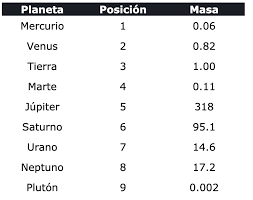
\includegraphics{figuras/tabla-ejemplo.png}\\
    {\textit{\small Fuente: } \textit{\small Autores por apellido (año). Titulo del documento de donde se copio la figura.}}
    \label{Tabla: Tabla ejemplo 2}
    \addcontentsline{lot}{table}{Tabla \arabic{cap2}.\arabic{tabla}: \descripcion}
    \addtocounter{tabla}{1}
\end{table}
% \label nos permite referenciar la tabla/figura en otra parte del documento.

Lorem ipsum dolor sit amet, consectetur adipiscing elit, sed do eiusmod tempor incididunt ut labore et dolore magna aliqua. Ut enim ad minim veniam, quis nostrud exercitation ullamco laboris nisi ut aliquip ex ea commodo consequat. Duis aute irure dolor in reprehenderit in voluptate velit esse cillum dolore eu fugiat nulla pariatur. Excepteur sint occaecat cupidatat non proident, sunt in culpa qui officia deserunt mollit anim id est laborum.
%-------------------------------------------------------------------------
% Titulo de ejemplo 2.2
\section{2.2 Titulo de ejemplo 2}
Lorem ipsum dolor sit amet, consectetur adipiscing elit, sed do eiusmod tempor incididunt ut labore et dolore magna aliqua. Ut enim ad minim veniam, quis nostrud exercitation ullamco laboris nisi ut aliquip ex ea commodo consequat. Duis aute irure dolor in reprehenderit in voluptate velit esse cillum dolore eu fugiat nulla pariatur. Excepteur sint occaecat cupidatat non proident, sunt in culpa qui officia deserunt mollit anim id est laborum.

% Modificar "\newcommand{\descripcion}{....} para describir el contenido de la tabla.
% Modificar la fuente según corresponda. 
\begin{table}[H]
    \centering
    \newcommand{\descripcion}{Descripción de la tabla.}
    \caption*{Tabla \arabic{cap2}.\arabic{tabla}: \descripcion}
    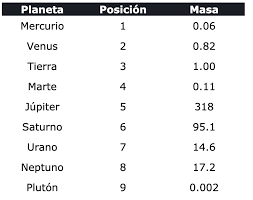
\includegraphics{figuras/tabla-ejemplo.png}\\
    {\textit{\small Fuente: } \textit{\small Autores por apellido (año). Titulo del documento de donde se copio la figura.}}
    \label{Tabla: Tabla ejemplo 3}
    \addcontentsline{lot}{table}{Tabla \arabic{cap2}.\arabic{tabla}: \descripcion}
    \addtocounter{tabla}{1}
\end{table}
% \label nos permite referenciar la tabla/figura en otra parte del documento.

%-------------------------------------------------------------------------
% Titulo de ejemplo 2.3
\section{2.3 Titulo de ejemplo 3}
Para escribir palabras y sus definiciones con una sangría después de los dos puntos, puedes utilizar el entorno de lista 'description' de LaTeX.

Puedes ajustar el espaciado entre la deinifición y los 2 puntos, y la sangría según tus preferencias utilizando los comandos labelwidth y leftmargin dentro del entorno description.
Por ejemplo:

\begin{description}[labelwidth=1.2cm, leftmargin=1.5cm]
\item[ESIG]: Encargado del sistema integrado de gestión plantas de alimentos Agrosuper.
\item[EPS]: Encargado del sistema integrado de gestión Planta.
\item[HACCP]: Siglas en inglés Hazard Analysis \& Critical Control Points, que significan Análisis de Peligros y Puntos Críticos de Control.
\item[MSIG]: Manual del Sistema Integrado de Gestión.
\item[R\&A]: Responsabilidad y autoridad.
\item[SGA]: Sistema de Gestión Ambiental basado en la norma ISO 14001:2015.
\item[SGS]: Sistema de Gestión de Salud y Seguridad Ocupacional basado en la norma ISO 
 45001: 2018.
\item[SGC]: Sistema de Gestión de Calidad basado en la norma ISO 9001:2015.
\item[SGIA]: Sistema de gestión de la inocuidad de los alimentos basado en la norma ISO 
 22000:2018.
\item[PPR]: Programa de prerrequisitos.
\item[PPRO]: Programa de prerrequisitos Operativos.
\item[SIG]: Sistema Integrado de Gestión, conformado por las normas ISO 9001:2015, ISO 
 14001:2015, ISO 45001:2018 e ISO 22000:2018.
\item[PDI]: “Pellets Durability Index” en inglés, acrónimo para determinar dureza del alimento, esta debe resistir íntegramente hasta el comedero del ave. 
\item[OPA]: “Optimización de Proceso Animal” Buscar de manera organizada y sistematizada 
 un animal óptimo para la rentabilidad del negocio.
\end{description}

En este ejemplo, el ancho del espacio para los términos se ha establecido en 1.2cm (labelwidth) y la sangría se ha establecido en 1.5cm (leftmargin). Puedes ajustar estos valores según tus necesidades.

\textbf{Lo mismo que antes, pero poniendo los 2 puntos dentro de los corchetes (no son considerados en el espaciado). Puede elegir la opción que más prefiera.}

\begin{description}[labelwidth=1.3cm, leftmargin=1.5cm]
\item[ESIG:] Encargado del sistema integrado de gestión plantas de alimentos Agrosuper.
\item[EPS:] Encargado del sistema integrado de gestión Planta.
\item[HACCP:] Siglas en inglés Hazard Analysis \& Critical Control Points, que significan Análisis de Peligros y Puntos Críticos de Control.
\item[MSIG:] Manual del Sistema Integrado de Gestión.
\item[R\&A:] Responsabilidad y autoridad.
\item[SGA:] Sistema de Gestión Ambiental basado en la norma ISO 14001:2015.
\item[SGS:] Sistema de Gestión de Salud y Seguridad Ocupacional basado en la norma ISO 
 45001: 2018.
\item[SGC:] Sistema de Gestión de Calidad basado en la norma ISO 9001:2015.
\item[SGIA:] Sistema de gestión de la inocuidad de los alimentos basado en la norma ISO 
 22000:2018.
\item[PPR] Programa de prerrequisitos.
\item[PPRO:] Programa de prerrequisitos Operativos.
\item[SIG:] Sistema Integrado de Gestión, conformado por las normas ISO 9001:2015, ISO 
 14001:2015, ISO 45001:2018 e ISO 22000:2018.
\item[PDI:] “Pellets Durability Index” en inglés, acrónimo para determinar dureza del alimento, esta debe resistir íntegramente hasta el comedero del ave. 
\item[OPA:] “Optimización de Proceso Animal” Buscar de manera organizada y sistematizada 
 un animal óptimo para la rentabilidad del negocio.
\end{description}

\textbf{SI DESEA ESCRIBIR EN EL TEXTO UN AMPERSAND (\&) DEBE HACERLO PONIENDO UN BACKSLASH (\textbackslash) ANTES DEL AMPERSAND, YA QUE SON CONSIDERADOS CARACTERES DE TABULACIÓN DE ALINEACIÓN EN LATEX. AL IGUAL QUE SI QUISIERA PONER UN PORCENTAJE (\%), YA QUE ESTOS SE UTILIZAN PARA HACER COMENTARIOS}